\section{ SR0012US23 }


\subsection{Meta}

    \textbf{Title:}
    Applications of Artificial Intelligence in the Radiology Roundtrip: Process Streamlining, Workflow Optimization, and Beyond

    \begin{table}[H]
        \centering
        \begin{tabular}{|c|c|c|c|c|c|c|c|c|}
            \hline
                \textbf{Rank} & \textbf{Grasp} & \textbf{Grade} & \textbf{Type} & \textbf{Outcome} & \textbf{Domain} & \textbf{COV19} & \textbf{CoI} & \textbf{DB} \\
            \hline
                1 & 85\% & C & A & P & B & Yes & Yes & No \\
            \hline
        \end{tabular}
        \caption{Reference's metadata}
        \label{tab:SR0012US23}
    \end{table}

\subsection{Summary}
    Kevin Pierre et al. \cite{x076} proposed a general overview of existing AI applications in radiology. The review highlights many examples; however, only two examples are somehow related to medical resource scheduling: radiology screening scheduling and image prioritisation for more efficient reporting and diagnostic time. The structure of the study can be improved. The authors praise the benefits of the AI approaches and do not mention the cons of the implemented solutions or possible ethical issues of exposing electronic medical data to machine learning algorithms. The work was conducted in collaboration with Nuance Communications Inc. and GE Healthcare, and has acted as a speaker or consultant for these entities.

\subsection{Notes}
    \begin{itemize}
        \item Picture Archiving and Communication System (PACS);
        \item Clinical Decision Support (CDS);
        \item Appropriate Use Critaria (AUC)-CDS model;
    \end{itemize}


\subsection{Reading}
    \textbf{Abstract:}
    The authors outline benefits of using AI in the radiology which are beyond diagnostic practicies.
    
    \textbf{Objectives:}

    
    \textbf{Page 1:}
    The emphasis in the introductio is on the ML approaches to "learn" in comparison with the traditional computational methods.
    
    \textbf{Page 2:}
    The standart approaches to solve radiology issues some times even does not consider need of a patient, when data driven methods like Natural Language Processing (NLP) has potential to work from data and therefore automatically be more practial in the real hospitals, not just in simulations.
    \begin{figure}[H]
        \centering
        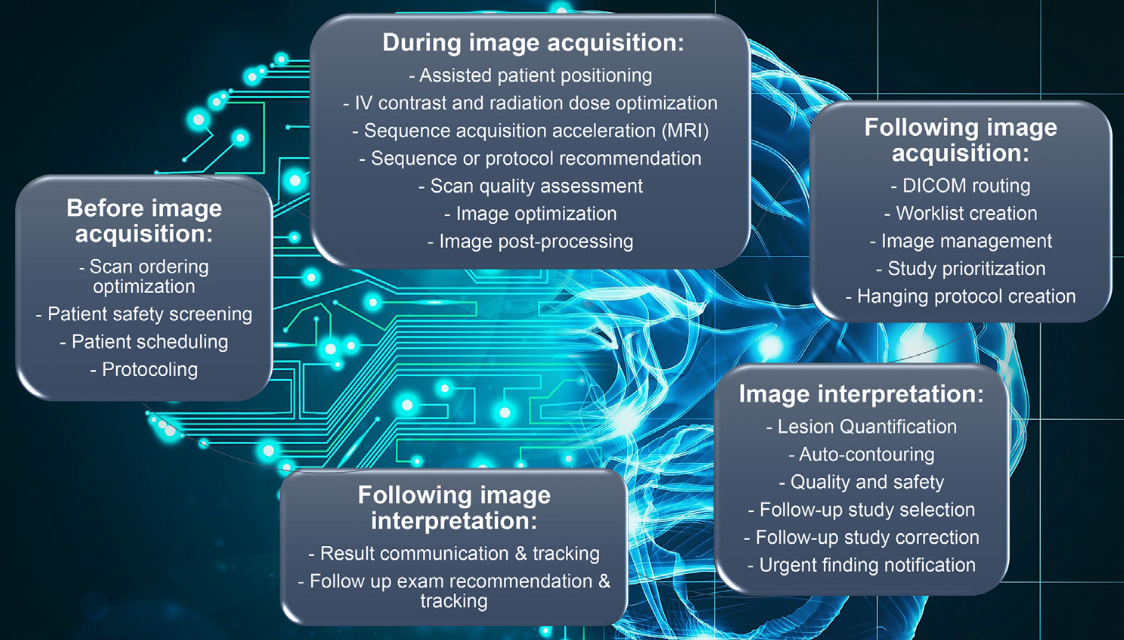
\includegraphics[width=1\textwidth]{figures/SR0012US23/fig1.png}
        \caption{Application of AI in radiology from \cite{x076}.}
        \label{fig1:SR0012US23}
    \end{figure}

    \textbf{Page 3:}
    This page provides some information on how imaging diagnostics in radiology works, possible analysis methods, and related little to the methods themself.
    \begin{figure}[H]
        \centering
        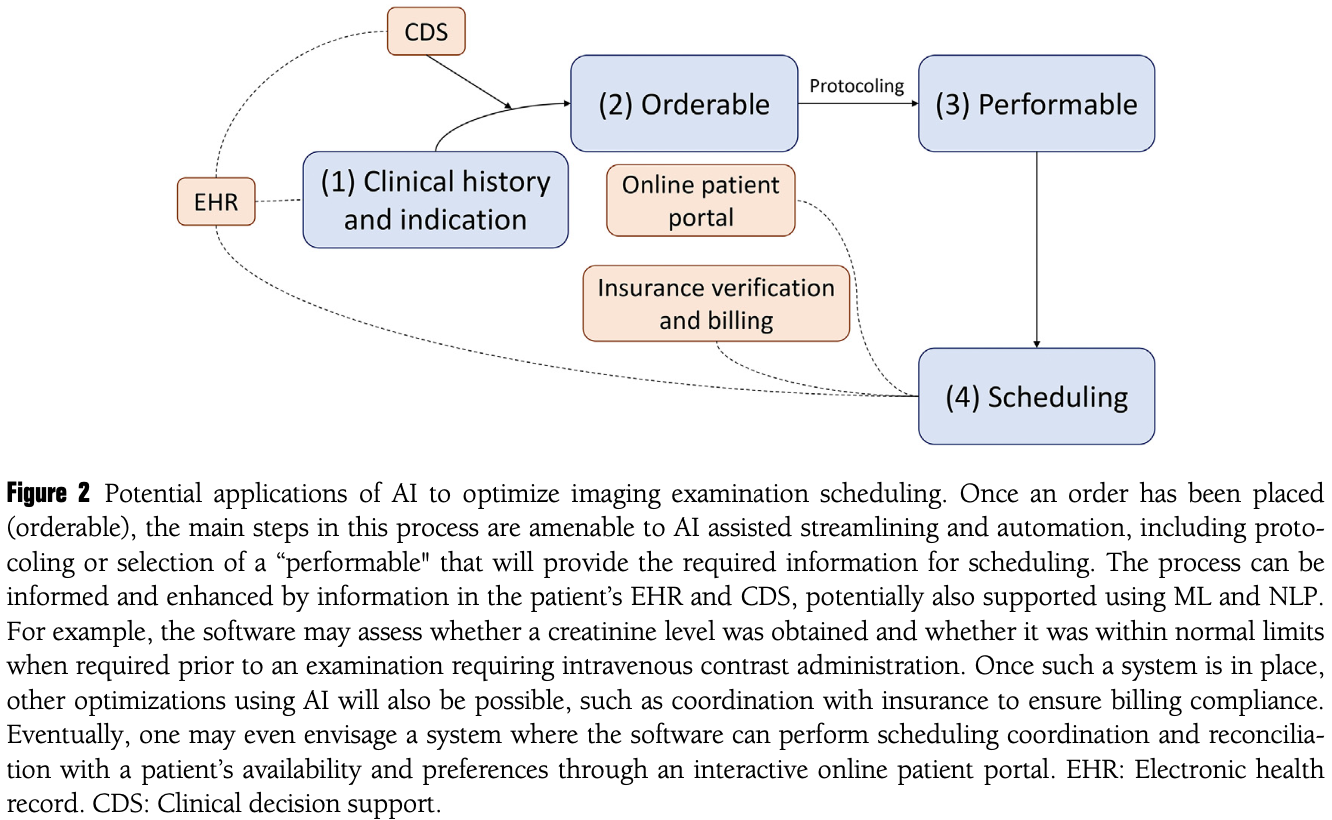
\includegraphics[width=1\textwidth]{figures/SR0012US23/fig2.png}
        \caption{Structure of a potential AI application in Radiology from \cite{x076}.}
        \label{fig2:SR0012US23}
    \end{figure}

    \textbf{Page 4:}
    In the first part of this page, the implementation an AI system was descriped. This sistem will flag inappropriate screenings or tests for patients due to alergies or/ and implants incompatible with the screening equipment. On the rest of the page, the protocoling of radiology procedures was describer. The radiologist may spend unnesessaty working hours on protocoling the radiology results wich is usually follow standart set of rules. There is known applications of AI where the NLP can relativelly accuarate and consistant make protocols for radiology screening. 

    \textbf{Page 5:}
    Efficient scheduling is an important aspect of the radiology patient flow. There is a place for an AI implementation. The positioning of an equipment during the scanning can be an issue. There are commersial AI systems which can solve this issue lieaing to enhanced screening result and lesser radiation exposion for patients. In addition, another ML model can adjust an optimal IV contrast radiation dosage for smaller exposior and sufficient screening outcome. Going even further, specialised Convolutionary Neural Networks can denose underexposed  images minimising the chance of repetative scanning.
    
    \textbf{Page 6:}
    The ML models can optimise workload by establishing the priorities for screens in the queue. Furthermore, the segmentation of the radiology images help identify the diagnosis for patients.
    
    \textbf{Page 7:}
    The AI tools system are also used to improve reporting, also workflow by notifying specialists about some required work to finish on rediolofy images. Other applications of the AI solutions contain educational purposes like providing a feedback on the quality of a radiological report.
    \begin{figure}[H]
        \centering
        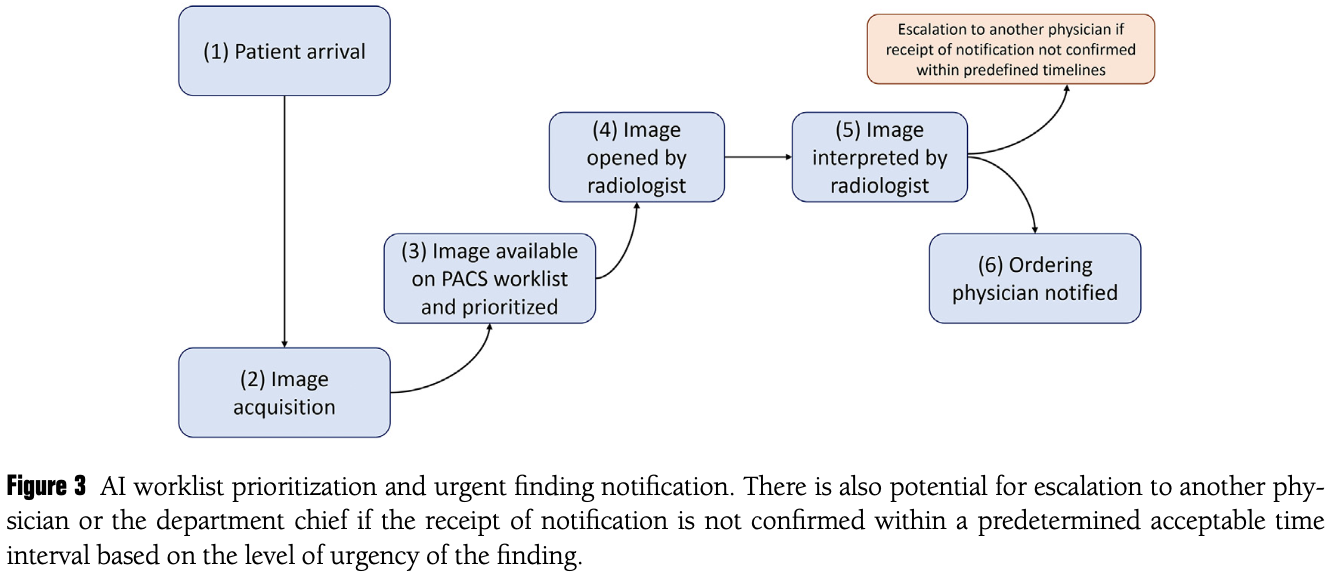
\includegraphics[width=1\textwidth]{figures/SR0012US23/fig3.png}
        \caption{AI worklist prioritisation from \cite{x076}.}
        \label{fig3:SR0012US23}
    \end{figure}

    \textbf{Page 8:}
    Quality assurance and Patient Safety: repeats the previuse applications. Billing and Comliance: by increasing radiology care efficiency thus reducing its costs. Miscellaneous Applications: lists other less investigated applications of AI in radiology.
    
    \textbf{Conclusion:}
    Standart computational methods are good but AI approaches are better.